\subsection{Reader Application}

For this component of the system we will also be using \textbf{Threat Modelling}, \textbf{focusing on Assets}. We decided that this approach is the best due to the same reasons as the mID application. Alongside this strategy, we are going to use the \textbf{STRIDE} approach complemented with a \textbf{Data Flow Diagram}.

\subsubsection{Focusing on Assets}

When we are Focusing on Assets while searching for potential threats in our system, it is important to think about 3 topics: \textbf{Things attackers want}, \textbf{Things you want to protect}, and \textbf{Stepping stones to either of these.} Considering our mID Reader, we answered these topics:

\textbf{Things attackers want}
\begin{itemize}
    \item Steal information that the reader requests
    \item Disrupt/sabotage service
    \item Add/Remove data to the identification requests
\end{itemize}

\textbf{Things you want to protect}
\begin{itemize}
    \item Data Integrity
    \item Service Reliability/Trustworthiness
\end{itemize}

\textbf{Stepping stones to either of these}
\begin{itemize}
    \item Use secure authentication
    \item Use secure communication channels
    \item Data encryption
\end{itemize}

\subsubsection{System Modelling}

The best way to understand what can go wrong with the mID Reader is to understand what it does. To do so, we will be using a \textbf{Data Flow Diagram} to represent this part of the system as well as it's interactions.

\begin{figure}[ht!]
 	\centering
 	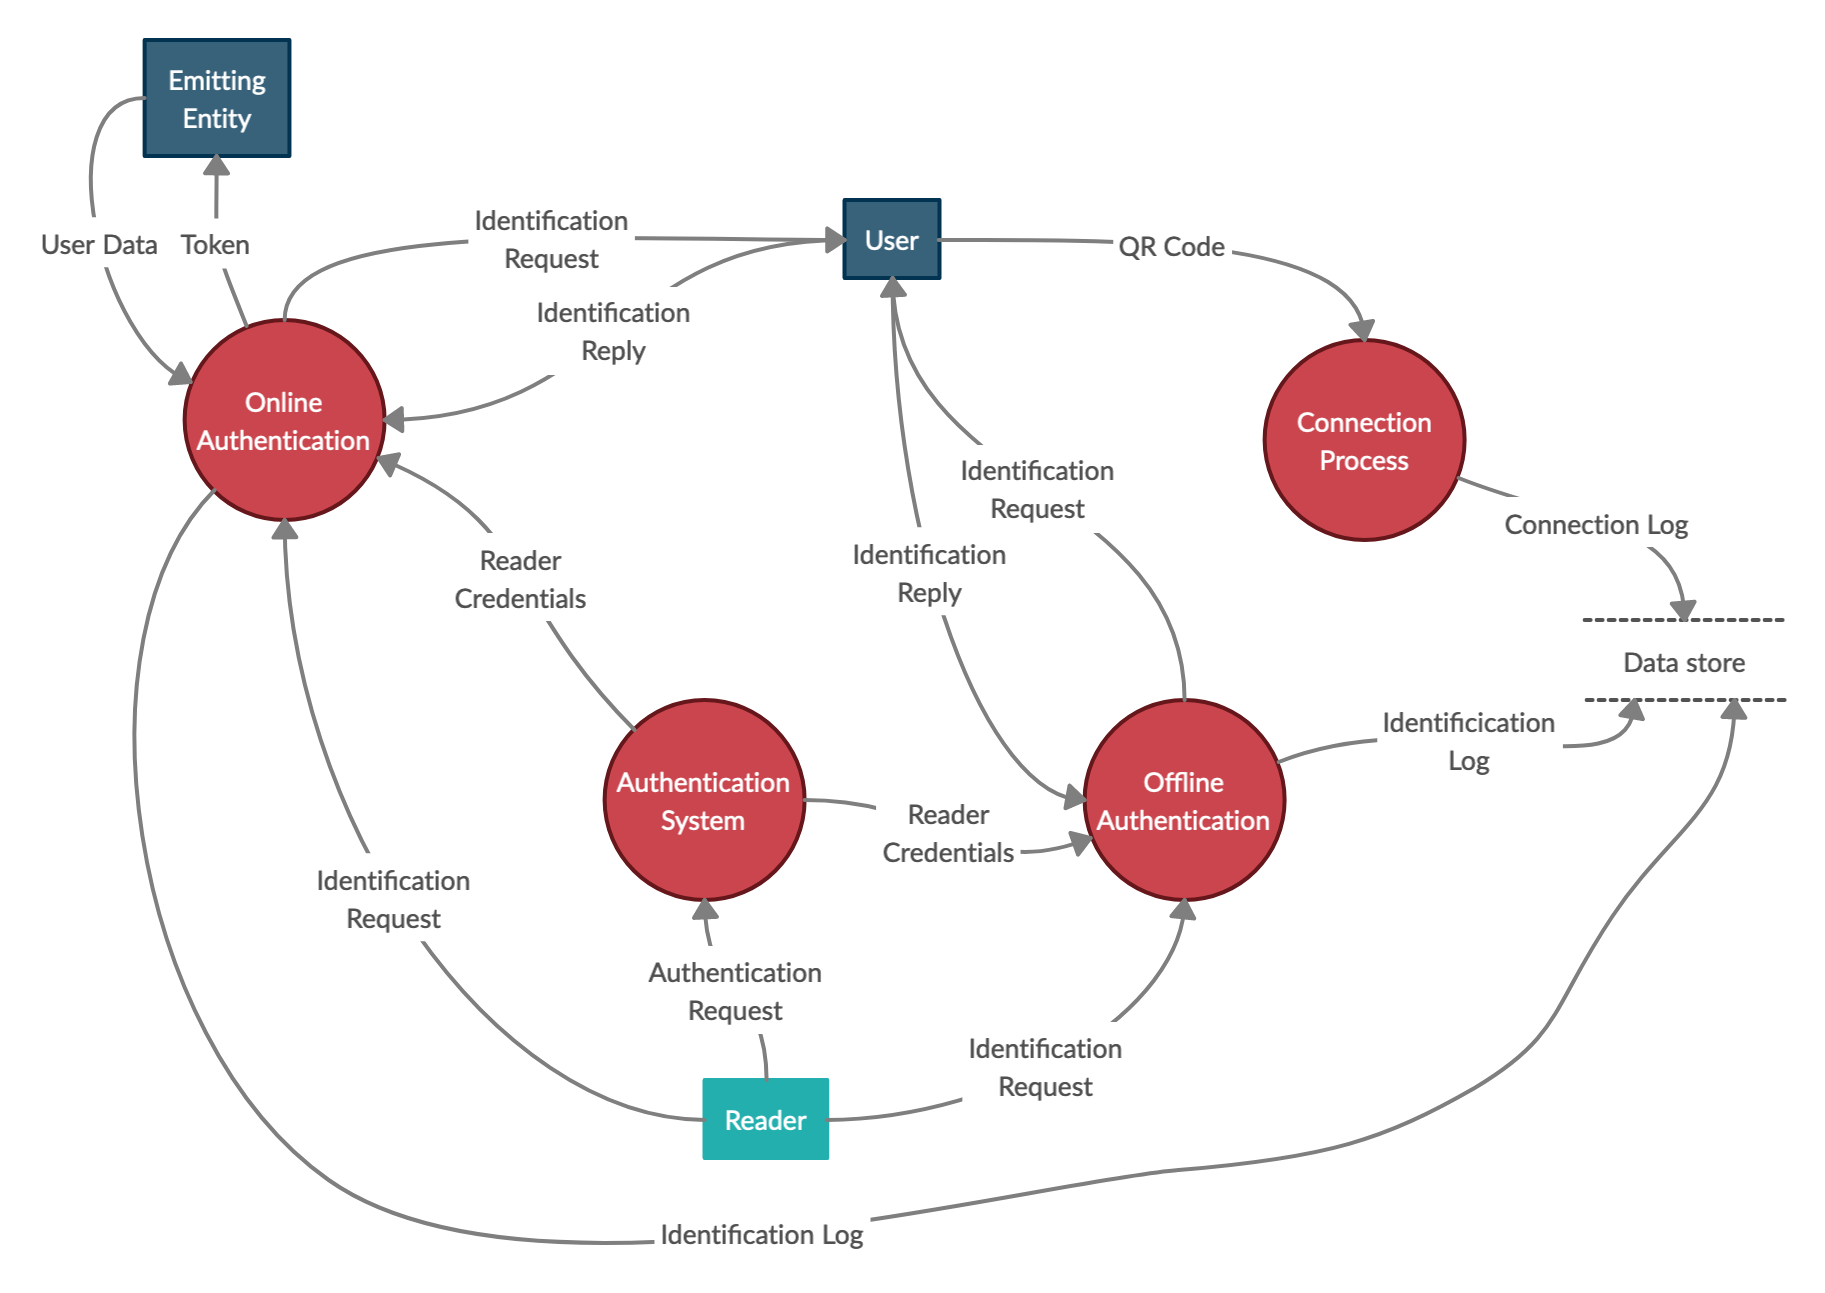
\includegraphics[width=0.8\linewidth]{img/mIDReaderDFD.png}
 	\caption{mID Reader Data Flow Diagram}
 \end{figure}
 
 We represented other elements of the system such as the User and Emitting Entity as external entities in order to better represent our communication with them, and, the local storage of the device was represented as a Data store.

\subsubsection{Finding Threats}

With our Data Flow Diagram done, we are now able to analyze it and find threats in a more streamlined way. In order to find the relevant threats, we will be using the STRIDE methodology:

\subsubsection{STRIDE}

\textbf{Spoofing}
\begin{itemize}
    \item The communication with the User is vulnerable to Spoofing. This occurs because when we receive identification fields, we have no way of guaranteeing that they belong, in fact, to the User that is in front of us. This situation could also be mitigated with the addition of a Public Key Infrastructure\cite{pki}. With the PKI we can verify the signature of the incoming identification data.
    \item The communication with the Emitting Entity is also lacking protection against Spoofing. For example, when we use a token to get a certain set of identification data we have no guarantee that it has been, in fact, sent by a trusted entity, and not by an attacker. Since this problem consists on the same nature of the last one, it can also be solved by using a PKI\cite{pki}.
\end{itemize}

\textbf{Tampering}
\begin{itemize}
    \item The local storage on the device where the mID Reader is located lacks protection since these devices are generic Android or iOS smartphones. These lack of specific protection could lead to an attacker being able to make changes in the logs, compromising our systems integrity. These attacker can be external attackers or even the user of the Reader Application. By encrypting the local storage on the mID Reader we could prevent these unwanted actions.
    \item Since we mostly rely on wireless communication there exists the possibility of an attacker modifying data flowing over the network. To prevent this, a good idea would be to work on encryption and signature of messages sent to the user, and use TLS\cite{tls} and HTTPS for communications with the backend. With this, we could prevent an attacker from adding/modifying data that is being transmitted.
\end{itemize}

\textbf{Repudiation}
\begin{itemize}
    \item Since we have no way of guaranteeing the authenticity of an entity's identity, we have no way of maintaining non-repudiation in our system. To avoid that, and as seen before, a PKI\cite{pki} would be useful to have signatures that uniquely identify an entity.
    \item The lack of protection on our local storage allows an attacker to modify our log files, which compromises the non-repudiation property of our system that we want. Despite also being a Tampering threat, this also falls in the Repudiation category. Luckily, it can be fixed with the same solution, by encrypting local storage.
\end{itemize}

\newpage

\textbf{Information Disclosure}
\begin{itemize}
    \item Following on the topic of local storage and its lack of protection, this also leads to the possibility of an attacker accessing the logs and extracting information from our system. In order do prevent this, encrypting the local storage would be a good idea.
    \item The communication channels with the emitting entity and the mID Application of the user are done over the network or BLE, NFC and WiFi-Aware. These communication channels do not offer protection against an attacker intercepting traffic and accessing information. To prevent this, the implementation of a security layer on these channels would be recommended. TLS\cite{tls} and HTTPS would be a good suggestion for TCP/IP channels, while for the others we could encrypt messages and sign them using our PKI\cite{pki}.
    \item One thing that we want to prevent in our system is that the reader or any kind of attacker may be able to add fields to the Authorization Token. To prevent this it would be a good idea to make use of the PKI\cite{pki} that we already mentioned, and encrypt the token after its creation, and decrypt it when it arrives on the backend only. Given this, we prevent the modification of the token to get more information that the user authorized.
\end{itemize}

\textbf{Denial of Service}
\begin{itemize}
    \item By not checking the origin of incoming information from users, or responses from the emitting entity, we are vulnerable to an attacker trying to flood the reader. This could be avoided by implementing content filtration. We could use the already suggested PKI\cite{pki} to discard incoming data with invalid signatures.
    \item In addition to flooding the reader, an attacker may try to fill the data store on the reader device in order to disrupt the service. The above mentioned filtration using the PKI\cite{pki} could be used to mitigate this problem. By adding a rule that checks the incoming data size, we could discard suspicious sizes.
\end{itemize}


\newpage

\textbf{Elevation of Privilege}
\begin{itemize}
    \item As seen on the mID Application, the local storage on the device is vulnerable to an attacker modifying bits on disk with the purpose of running unauthorized commands. This could also be solved by encrypting local storage.
\end{itemize}


\subsubsection{Risk Analysis}

With the help of the STRIDE methodology we were able to search for vulnerabilities that the mID Reader may encounter when in use. Unfortunately, resources are limited and there are vulnerabilities that are more important and should be addressed first. With that in mind, we tried to evaluate what should be implemented/focused on first. For that process of evaluation we tried to make a \textbf{Risk Analysis}, which involves analyzing the probability of something happening with the impact that this could have. We added also the weight of one solution fixing multiple problems.
Given this, and after making the proper analysis, we decided that from the previous solutions we proposed, the ones that should be focused on first are: the addition of a \textbf{Public Key Infrastructure} to the system both for encryption and data signature, and the use of \textbf{Transport Layer Security} in communications. By adding these functionalities to the system, a big part of the listed vulnerabilities could be mitigated.